% arara: pdflatex
\documentclass{beamer}
\usepackage[latin1]{inputenc}
\usetheme{PaloAlto}
\usepackage{standalone}
\usepackage{tikz}
\usetikzlibrary{positioning}
%Does someone have a theme they like or one they created for PCC?

\title{Mathematics SAC Program Review}
\institute{Portland Community College}
\date{January 31, 2014}
\begin{document}

\begin{frame}
\titlepage
\end{frame}

%Let me know if there is anything out of place or something you think should be moved to another page. 

\begin{frame}{Highlights from the last 5 years}

\begin{itemize}
%Is there a good way to reference the page numbers in the larger document? I thought it would be nice to have parenthetical page numbers. 

\pause \item Creation of Developmental Math Subcommittee
	\begin{itemize}
	\pause\item More meaningful outcomes
	\pause\item Research driven
	\pause\item Large faculty involvement
	\pause \item Large scale curriculum reform (future goal)
	\end{itemize}

\pause \item Study Skills Workbook
\pause \item Social Justice Workgroup
\pause \item Mathematics Accesibility Study
\pause \item WeBWorK
	\begin{itemize}
	\pause \item Accesibility
	\pause \item Free
	\pause \item Problem Library Development
	\pause \item Future Developments
	\end{itemize}

\pause \item Other Technology innovations in the classroom
	\begin{itemize}
	\pause \item ALEKS
	\pause \item GeoGebra
	\end{itemize}

\end{itemize}
\end{frame}

\begin{frame}{Highlights}
\begin{itemize}
\pause \item Formation of Math SAC Distance Learning Standing Subcommittee.
\pause \item Formation of Math Learning Assessment Subcommittee
	\begin{itemize}
	\pause \item Assessment Team
	\pause \item Action Team
\end{itemize}

\pause \item Faculty committed to professional development and serving the college. 
	\begin{itemize}
	\pause \item Multiple college wide committees (including several chairs)
	\pause \item Conference attendance
	\pause \item Memberships in professional organizations
	\pause \item Improved Dual Credit Relationships
	\end{itemize}

\end{itemize}
\end{frame}

\begin{frame}{Highlights}
\begin{itemize}

\pause \item Enrollment growth in LDC courses. 
\pause \item Curricular Changes
	\begin{itemize}
	\pause \item  Condensed MTH 111B and MTH 111C into MTH 111. 
	\pause \item MTH 105 replaced MTH111A and increased enrollment.  
	\pause \item MTH 111H created. 
	\pause \item All classes with MTH prefix are now part of the MTH SAC. 
	\pause \item MTH 243 credit change and future pre-requisite change. 
	\pause \item MTH 84 (LaTeX) course created
	\end{itemize}
\pause \item ALC and AMP
	\begin{itemize}
	\pause \item ALC (Alternative Learning Centers) courses allow students the opportunity to work on the math they need to work on for credit (but not for pre-requisites). 
	\pause \item AMP (Accelerated Math Placement) allows students to review material and gives them the chance to take the placement exam again for (possibly) higher placement. 
	\end{itemize}

\end{itemize}
\end{frame}
 
\begin{frame}{The Future of the Math SAC}

%insert flow chart here
%maybe this will work once it gets compiled?

\makebox[\textwidth][c]{%
  % arara: pdflatex
% !arara: indent: {overwrite: yes}
\documentclass[tikz]{standalone}

\usepackage{tikz}
\usetikzlibrary{positioning}

\begin{document}
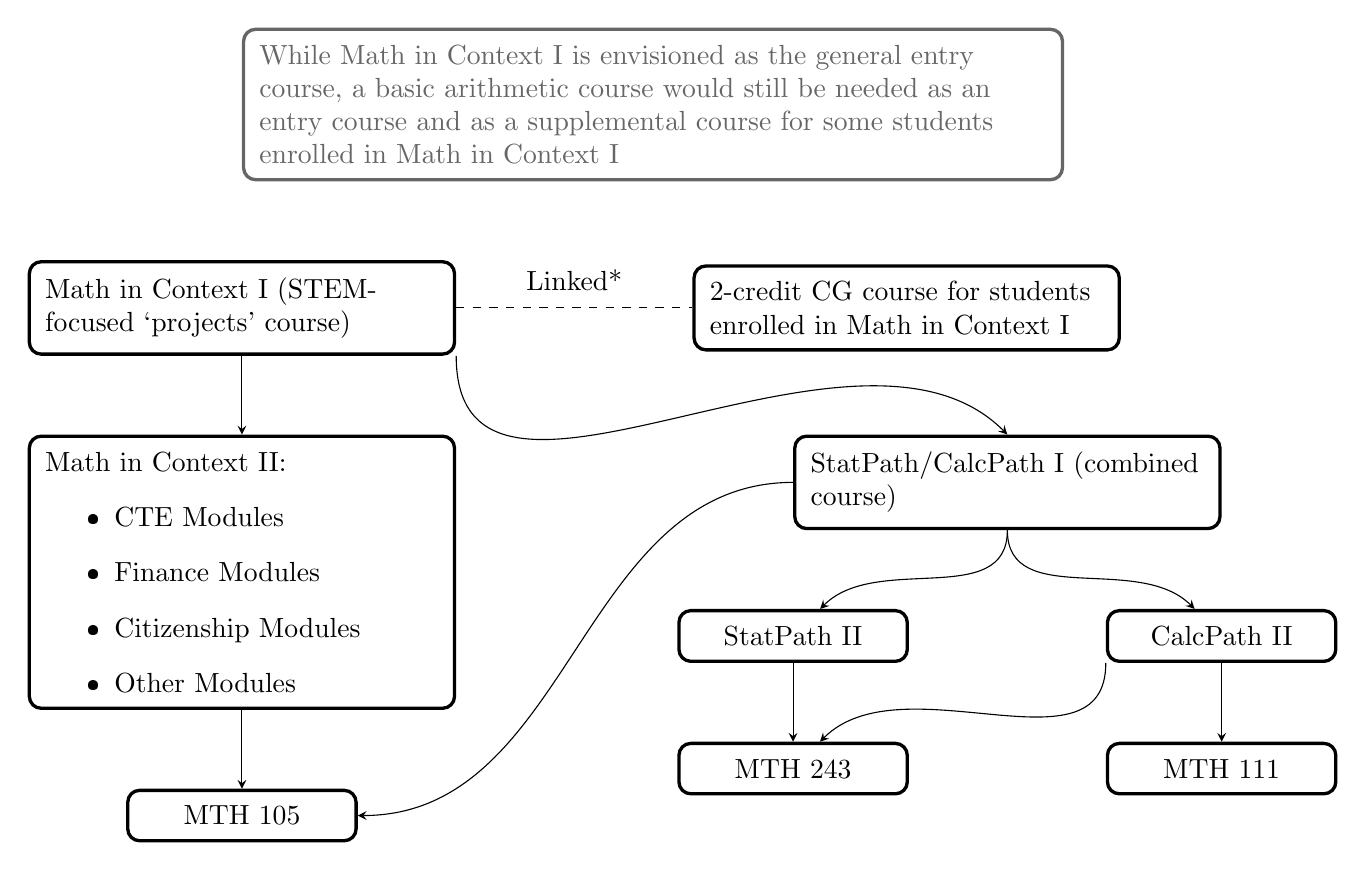
\begin{tikzpicture}[
		>=stealth,
		every node/.append style={
			draw=black,
			rounded corners=1ex,
			very thick,
			inner sep=.2cm,
		},
		wide/.style={text width=5cm},
		narrow/.style={text width=2.5cm,align=center},
	]
	\node[text width=10cm,black!60] (entrycourse) at (0,0) {While Math in Context I is envisioned as the general
		entry course, a basic arithmetic course would still be needed as an entry course
	and as a supplemental course for some students enrolled in Math in Context I};
	% left side of the picture
	\node[wide] (context1) [below=of entrycourse.south west]{Math in Context
	I (STEM-focused `projects' course)};
	\node[wide] (cgcourse) [right =3cm of context1]{2-credit CG course for students enrolled in Math in Context I};
	\node[wide](context2) [below=of context1]{
		Math in Context II:
		\begin{itemize}
			\item CTE Modules
			\item Finance Modules
			\item Citizenship Modules
			\item Other Modules
		\end{itemize}
	};
	\node[narrow] (math105) [below=of context2]{MTH 105};
	% right side of the picture
	\node[wide] (combined) [xshift=7cm,below=of context1.south east] {StatPath/CalcPath I (combined course)};
	\node[narrow] (stat2) [below=of combined.south west] {StatPath II};
	\node[narrow] (calc2) [below=of combined.south east] {CalcPath II};
	\node[narrow] (math243) [below=of stat2] {MTH 243};
	\node[narrow] (math111) [below=of calc2] {MTH 111};
	% draw the connection lines
	\draw[dashed] (context1)--(cgcourse) node [draw=none,pos=0.5,anchor=south]{Linked*};
	\draw[->] (context1.south east) to[out=270,in=135] (combined.north);
	\draw[->] (context1) -- (context2);
	\draw[->] (context2) -- (math105);
	\draw[->] (combined) to[out=270,in=45] (stat2);
	\draw[->] (combined) to[out=270,in=135] (calc2);
	\draw[->] (combined.west) to[out=180,in=0] (math105.east);
	\draw[->] (stat2) -- (math243);
	\draw[->] (calc2) -- (math111);
	\draw[->] (calc2.south west) to[out=270,in=45] (math243);
\end{tikzpicture}
\end{document}

  }

*Every student in a given section of Math in Context I 
would also be enrolled in a common section of the CG 
course.  The instructors of a given pair of courses 
would work in a collaborative fashion and ideally visit 
one another's classes, especially the first week. 

Unlinked sections of the CG course would be offered 
for entry level DE mathematics students whose initial 
placement is `above' Math in Context I.  Students who 
pass Math in Context I but not the attendant CG course 
might be required to retake the course.

\end{frame}

\end{document}
